\chapter{Introduction}\label{ch: intro}

% Intro with Muybridge story
In 1962 and 1964, the Nobel Prizes in Chemistry~\cite{Nobel1964, Nobel1972}
were awarded to crystallographers John C. Kendrew~(1917--1997), Max F. Perutz~(1914--2002),
and Dorothy C. Hodgkin~(1910--1994) for their work in determining for the first time
the 3D~structure of several important macromolecules.%
\footnote{Kendrew and Perutz solved by X-ray diffraction~(XRD)
the structure of myoglobin~\cite{Kendrew1960} and haemoglobin~\cite{Perutz1960} respectively
while Hodgkin did so for cholesterol~\cite{Carlisle1945}, penicillin~\cite{Hodgkins1949},
vitamin B$_{12}$~\cite{Hodgkins1949}, and insulin~\cite{Hodgkins1949}.}
In response, enzymologists Herbert Gutfreund and Jeremy R. Knowles~\cite{Gutfreund1967} noted that
``making a model of a horse from photographs does not necessarily tell us how fast it can run,''
an apocryphal reference to the 1878 work \textit{The Horse in Motion} of Eadweard Muybridge ---
the earliest example of high-speed photography
wherein the all four hooves of a horse in mid-gallop were conclusively shown to be off the ground,
as seen in Fig.~\ref{fig: intro-muybridge}a.
%
This is a reminder that a mechanistic understanding of the physics and chemistry of a molecular system
in action requires direct observation of its component atoms on the relevant spatio-temporal scales,
i.e.~a `molecular movie' with sub-angstrom ($< 10^{-10}$~m) spatial
and femtosecond~($10^{-15}$~s) temporal resolutions.
%
An experimental method that can deliver such results is `ultrafast electron diffraction'~(UED).

% Figure: Muybridge's Horse in Motion
\begin{figure}[ht!]
  \centering
  \includegraphics[width = \textwidth]{Figures/fig_intro_muybridge.pdf}
  \caption[Introduction to time-resolved crystallography.]{
    Introduction to time-resolved crystallography.
    (a)~\textit{The Horse in Motion}: `instantaneous photography' of the horse Sallie Gardner
    running at a gallop, in steps of ca.~40~ms and exposure of $<2$~ms,
    taken by Eadweard Muybridge in 1878~\cite{Muybridge1878}.
    (b)~Time and length scales of ultrafast structural dynamics~\cite{Krausz2009, Hada2013,
    Ischenko2017} relative to the speed of light; dashed lines show the de~Broglie wavelength
    and instrument response function~(IRF) time of the UED setup described in Sec.~\ref{sec: UED}.
    (c)~Protein Data Bank~(PDB) statistics showing the growth in the number of molecular structures
    solved by X-ray diffraction, nuclear magnetic resonance, and electron microscopy
    and diffraction~\cite{PDB2000}.
  }
  \label{fig: intro-muybridge}
\end{figure}

% UED
UED is as its name suggests: time-resolved crystallography by electron diffraction
with sub-picosecond time resolution (see Figs.~\ref{fig: intro-muybridge}b
and~\ref{fig: intro-scales}).
It is the culmination of a series of scientific breakthroughs and technological innovations
over the past century, from the discovery of the electron in 1897~\cite{Thomson1897}
to the invention of nanometer ultramicrotomy in 1950~\cite{Pease1981, Villiger1990},
chirped pulse amplification in 1985~\cite{Strickland1985}, and
radio-frequency compression of femtosecond electron bunches in 2007~\cite{vanOudheusden2007}.
%
Indeed, the technical development of UED, along with that of its XRD sibling, is an interesting story
and it has been covered extensively in several topical reviews
by leaders of the field~\cite{Glaeser1999, Zewail2006, Chergui2009, Hada2013, Carbone2012,
Centurion2016, Chergui2017, Spence2017, Ischenko2017} and the references therein.
%
Thus, this history%
\footnote{A more detailed account on the relevant fields beyond UED can be found in the books
\textit{Pathways to Modern Chemical Physics}~\cite{Califano2012} and
\textit{Early Days of X-ray Crystallography}~\cite{XRDBook}.} is briefly summarized
as a timeline in Fig.~\ref{fig: intro-timeline} in App.~\ref{ap: intro-timeline}.

% ms TR-XRD
% 1981: ns TR-XRD (Endert et al)
% 1996: ps TR-XRD (Bourgeois et al)
% 1997: fs TR-XRD (Rischel et al, Neutze et al)
% 2000,2006: diffraction before destruction (Hadju et al; Chapman et al)
% 1996: ns TR-XRD of myoglobin (Srajer et al)
% 2003: ps TR-XRD of myoglobin (Schotte et al)

% Figure, energy vs wavevector or wavelength (photons vs electrons vs neutrons vs ultrasound)

% Pathways to Modern Chemical Physics (Salvatore Califano)

% first X-ray absorption edge measured: 1913 by Maurice de Broglie cite Lytle1999.

% % First maser
% \cite{Gordon1954}
%
% % First laser (proposed)
% \cite{Schawlow1958}
%
% % First laser
% \cite{Maiman1960}
% \cite{Sugano2013}
% % 4A2, (t2g)3 -> 4T1 -> 4T2, (t2g)2(eg)1 -> 2E, (t2g)3 ----> 4A2 + hv
% % https://chemicalstructure.net/portfolio/ruby/
% % AMERICAN INSTITUTE OF PHYSICS CENTER FOR HISTORY OF PHYSICS LASER HISTORY PROJECT RECORDS
%
% % Critique of XFELs, pro-electrons
% \cite{Henderson1995, Henderson2002, Spence2017}
%
% % Recent review paper on Cryo-EM
% \cite{Merk2016}
%
% % Recent paper on electron diffraction limits (H atoms)
% \cite{Palatinus2017}
%
% % Electron diffraction history
% \cite{Gehrenbeck1978, Davisson1923, Born1927, Davisson1927, Thomson1927}
%
% % Quasicrystal via electron diffraction
% \cite{Shechtman1984, Levine1984}

% % Ptychography
% % Nature News and Views: A record-breaking microscope
% % Latest: Electron ptychography of 2D materials to deep sub-ångström resolution

\section{The Scientific Question}

The main focus of this thesis is to capture chemistry in action
by making molecular movies with UED.
%
The key question that is posed is not whether any ultrafast structural dynamics
can be elucidated this way. What is asked instead is:
%
\vspace{0.5\baselineskip}
%
\begin{center}
  \begin{minipage}{0.8\textwidth}
    Can the sub-angstrom and femtosecond atomic motions of \emph{large},
    \mbox{\emph{low-symmetry}}, and \emph{weakly scattering} molecules be resolved by
    \mbox{ultrafast} \mbox{electron} diffraction?
  \end{minipage}
\end{center}

\vspace{0.5\baselineskip}

% Figure: previous UED data analysis
\begin{figure}[ht!]
  \centering
  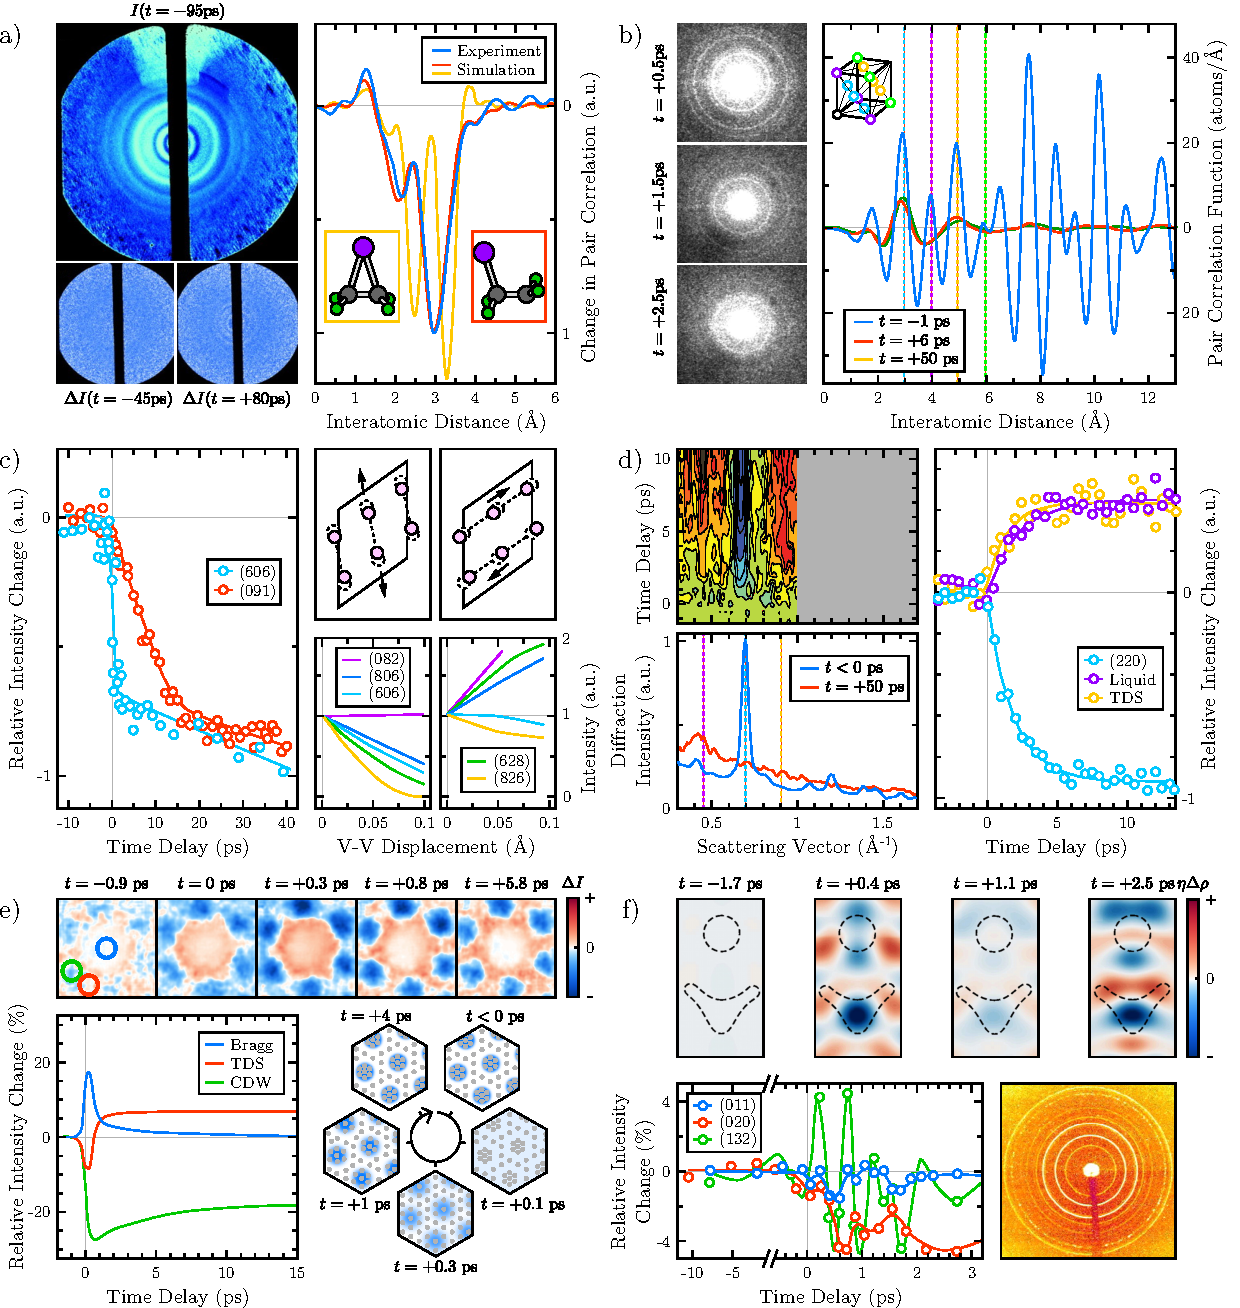
\includegraphics[width = \textwidth]{Figures/fig_intro_data.pdf}
  \caption[Making molecular movies by ultrafast diffraction.]{
    Making molecular movies by ultrafast diffraction:
    (a)~non-concerted elimination reaction in gas-phase $\mathrm{C_2 F_4 I_2}$;
    (b)~laser-induced melting of single-crystal aluminum;
    (c)~photoinduced phase transition in single-crystal {VO$_2$};
    (d)~laser-induced bond hardening of polycrystalline gold;
    (e)~optical suppression of charge density waves in single-crystal {1T-TaS$_2$};
    (f)~ultrafast charge transfer in powder KH$_2$PO$_4$.
    Adapted with permission from Refs.~\cite{Ihee2001, Siwick2003, Baum2007,
    Ernstorfer2009, Eichberger2010, Zamponi2012} respectively.
  }
  \label{fig: intro-data}
\end{figure}

% Describe previous UED works
Prior to my contributions in 2013,
several works in the literature have already answered the above question
in the affirmative for small molecules in the gas phase~\cite{Ihee2001},
highly symmetric materials~\cite{Baum2007, Eichberger2010, Zamponi2012},
and simple metals~\cite{Siwick2003, Ernstorfer2009}.
%
Some of their major results and approaches are summarized in Fig.~\ref{fig: intro-data}.
%
In Panel~(a), Ihee et~al~\cite{Ihee2001} determined the structure of a reaction intermediate
by calculating the change in pair correlation function from the difference diffraction pattern
and comparing it to that from two chosen structure models (`bridged' versus `classical').
%
In Panels~(b) and (d), Miller and co-workers~\cite{Siwick2003, Ernstorfer2009}
followed the laser-induced melting of two simple metals by directly interpreting
the time evolution of the correlation values of known atomic pairs
in a face-centered-cubic unit cell~\cite{Siwick2003} or the intensity of diffraction features
associated with the different phases (solid versus liquid) and
thermal diffuse scattering~(TDS)~\cite{Ernstorfer2009}.
%
In Panel~(c), Baum et~al~\cite{Baum2007} deduced the motion of the one asymmetric vanadium atom
in VO$_2$ crystals during its photoinduced phase transition
by considering the amplitude and sign of the intensity changes of 16 diffraction spots
and comparing them again to those calculated from the structure factor of
two likely structure models.
%
In Panel~(e), Eichberger et~al~\cite{Eichberger2010} observed the suppression and recovery
of charge density waves~(CDW) in the highly symmetric material {1T-TaS$_2$}
by observing the rise and fall in intensity of diffraction features associated with
the lattice order of the Ta~atoms (Bragg spots), disorder (inelastic background),
and the six-fold superlattice distortions caused by CDW (satellite spots).
%
Finally, in Panel~(f), Zamponi et~al~\cite{Zamponi2012} reconstructed the charge density distribution
of {KH$_2$PO$_4$} from powder XRD data by assuming that the 2D~inversion symmetries of the unit cell
are conserved and thus forcing the phase change of the structure factors
to always be either $0$ or $\pm \pi$.

% Caveats of above methods
In the above cases, the structural dynamics of the sample could be inferred so simply
because of the small number of asymmetric atoms.
%
As in Refs.~\cite{Ihee2001, Baum2007} and others,
such molecular systems have low degrees of freedom and thus
only a small number of structural ansatzes need to be tested.
%
Similarly, in highly symmetric crystals like simple metals~\cite{Siwick2003, Ernstorfer2009},
the space of interatomic distances is so sparse that
the atomic motions can be read out directly from peaks of the pair correlation function
calculated by a Fourier transform of the measured diffraction patterns.
%
In addition, the presence of conserved inversion symmetries,
as in Ref.~\cite{Zamponi2012} and similar works,%
\footnote{See Refs.~\cite{Zamponi2010, Woerner2010, Stingl2012, Zamponi2012b, Juve2013, Freyer2013}.}
means that there is not much a phase problem to solve:
the complex phase of the structure factors is therein fixed at $0$ or $\pm \unslant[-.2]\pi$.
%
Another simplifying consequence of these few-atom samples
is that they expectedly exhibit structural dynamics of low dimensionality
in terms of reaction coordinates;
most of the active atomic motions could be captured and discerned
by sampling only a small subset of diffraction spots in reciprocal space.
%
Lastly, the task of making molecular movies therein was made easier
by having the active atoms be strong scatterers --- e.g. V~\cite{Baum2007},
I~\cite{Ihee2001}, Ta~\cite{Eichberger2010}, Au~\cite{Ernstorfer2009}, Bi~\cite{Sciani2009} ---
which could afforded the higher signal-to-noise ratios~(SNR) necessary
for resolving subtle time-dependent changes in the diffraction data.

% Previous methods not applicable
The molecular systems whose results are described in this thesis
are non-trivial with respect to those studied prior in the literature.
%
They are mostly composed of weakly scattering carbon,
with ca.~$100$ atoms in a moderately sized unit cell%
\footnote{See App.~\ref{ap: cif} for their crystallographic information.} of lower symmetry,
chosen for the interesting photo-physics and chemistry that can be accessed
by laser excitation and acts as test~cases for proteins and other biological macromolecules
in more ambitious UED experiments of the future.
%
As such, these molecule movies cannot be made using the previously used tricks
and requires a new approach --- herein based on data science ---
that shall constitute the scientific question and answer of this thesis.

% Describe the phase problem of crystallography
% Figure: Cowtan's cat
% http://www.ysbl.york.ac.uk/~cowtan/fourier/coeff.html

% In the case of the experiment described in Sec.~\ref{sec: UED-AZA},
% 123,768 images --- $0.28$~TB --- were collected over 15 days.
% ($219.2$~kB/s)

% Streaking experiments (Carbone2012)
% Reflection experiments

% First paper on radial functions in electron diffraction (gas) \cite{Pauling1935, Debye1941}

% % 4th paradigm of science: data
% \cite{Agrawal2016}.


\section{Overview of Thesis}

% The goal of this thesis is to directly observe the ultrafast changes in structure of molecules
% during a chemical reaction using UED. In other words, it is to make
% a molecular movie with femtosecond time resolution and sub-angstrom spatial resolution.
% I will show that I have achieved this goal and made several significant contributions along the way,
% under the supervision of R. J. Dwayne Miller and in collaboration with many other colleagues.

Large portions of this thesis are based on works --- experiments and discussions ---
done in collaboration between several colleagues and me.
The results described herein have been previously published in the following articles:
%
\begin{itemize}
  \item M. Gao, C. Lu, H. Jean-Ruel, \underline{L. Liu}, A. Marx, K. Onda, S.-Y. Koshihara,
    Y. Nakano, X. Shao, T. Hiramatsu, G. Saito, H. Yamochi, R. R. Cooney, G. Moriena, G. Sciaini,
    and R. J. D. Miller,
    ``Mapping Molecular Motions Leading to Charge Delocalization with Ultrabright Electrons,''
    \textit{Nature}, vol.~496, pp.~343--346, 2013.

  \item H. Jean-Ruel, M. Gao, M. A. Kochman, C. Lu, \underline{L. Liu}, R. R. Cooney,
    C. A. Morrison, and R. J. D. Miller,
    ``Ring-Closing Reaction in Diarylethene Captured by Femtosecond Electron Crystallography,''
    \textit{J. Phys. Chem. B}, vol.~117, pp.~15894--15902, 2013.

  \item S. Manz, A. Casandruc, D. Zhang, Y. Zhong, R. A. Loch, A. Marx, T. Hasegawa,
    \underline{L. Liu}, S. Bayesteh, H. Delsim-Hashemi, M. Hoffmann, M. Felber, M. Hachmann,
    F. Mayet, J. Hirscht, S. Keskin, M. Hada, S. W. Epp, K. Fl\"{o}ttmann, and R. J. D. Miller,
    ``Mapping Atomic Motions with Ultrabright Electrons: Towards Fundamental Limits in Space-Time
    Resolution,'' \textit{Farad. Discuss.}, vol.~177, pp.~467--491, 2015.

  \item R. L. Field, \underline{L. Liu}, W. Gawelda, C. Lu, R. J. D. Miller,
    ``Spectral Signatures of Ultrafast Spin Crossover in Single Crystal
    [Fe\textsuperscript{II}(bpy)\textsubscript{3}](PF\textsubscript{6})\textsubscript{2},''
    \textit{Chem. Eur. J.}, vol.~22, pp.~5118--5122, 2016.

  \item Y. Jiang, \underline{L. Liu}, H. M. M\"{u}ller-Werkmeister, C. Lu, D. Zhang, R. L. Field,
    A. Sarracini, G. Moriena, E. Collet, and R. J. D. Miller,
    ``Structural Dynamics upon Photoexcitation in a Spin Crossover Crystal Probed
    with Femtosecond Electron Diffraction,''
    \textit{Ang. Chem. Int. Ed.}, vol.~56, pp.~7130--7134, 2017.

  \item \underline{L. Liu}, Y. Jiang, H. M. M\"{u}ller-Werkmeister, C. Lu, G. Moriena,
    M. Ishikawa, Y. Nakano, H. Yamochi, and R. J. D. Miller,
    ``Ultrafast Electron Diffraction Study of Single-Crystal
    (EDO-TTF)\textsubscript{2}SbF\textsubscript{6}: Counterion Effect and Dimensionality Reduction,''
    \textit{Chem. Phys. Lett.}, vol.~683, pp.~160--165, 2017.

  \item K. M. Krawczyk, R. L. Field, \underline{L. Liu}, M. Dong, A. Woolley, and R. J. D. Miller,
    ``Illuminating the Photoisomerization of a Modified Azobenzene Single Crystal
      by Femtosecond Absorption Spectroscopy,'' \textit{Can. J. Chem.}, vol.~97, pp.~488--495, 2019.

  \item Y. Jiang, \underline{L. Liu}, K. M. Krawczyk, A. Sarracini, J. S. Wentzell, Cheng Lu,
    R. L. Field, S. F. Matar, W. Gawelda, H. M. M\"{u}ller-Werkmeister, and R. J. D. Miller,
    ``Direct Observation of Nuclear Reorganization Driven by Ultrafast Spin Transitions,''
    2019 (under consideration).

\end{itemize}

In reflection of the multifaceted nature of my doctoral work,
this thesis is organized into a methods chapter (Ch.~\ref{ch: methods})
and several `science' chapters (Ch.~\ref{ch: UED-EDO}--\ref{ch: SCO})
that are each focused on the results reported in one of the above publications.

I will begin in Ch.~\ref{ch: methods} by describing the theoretical and experimental framework
of the two techniques used throughout these works:
transient absorption~(TA) spectroscopy and ultrafast electron diffraction.
I will give an overview of the physics of the relevant probe-matter interaction,
the experimental setup used to perform the measurements, and novel data analysis procedures that
I developed to extract weak signal from noisy datasets and reconstruct the relevant ultrafast dynamics
of the molecules under study.

In Ch.~\ref{ch: UED-EDO}, I will present experimental results on the ultrafast structural dynamics
of the family of molecules (EDO-TTF)\textsubscript{2}X, where X = PF\textsubscript{6}
and SbF\textsubscript{6}.
In the case of X = PF\textsubscript{6}, the experiment demonstrates that it is possible with UED to
resolve the atomic motions of an organic crystal as it reversibly undergoes
a photoinduced insulator-to-metal phase transition~\cite{Gao2013}.
The data analysis reveals the existence of a short-lived intermediate state whose formation involves
motions distinct from the thermal motions that drive later relaxation to the final state.
In the second half of the chapter, I will discuss results from a follow-up experiment,
where a much larger SbF\textsubscript{6} ion is substituted
for the PF\textsubscript{6} ion~\cite{Liu2017}. Here, I will examine the under-appreciated role
played by these spectator ions and focus on the consequences of this atomic replacement
on the structural dynamics of the EDO-TTF ions after photoexcitation.

In Ch.~\ref{ch: UED-DAE}, I will describe UED work on a class of organic molecules known
as diarylethenes (DAE)~\cite{Jean-Ruel2013}. This study focuses on directly observing
the photoinduced ring-closing reaction that occurs in this molecular system.
This photochemical process is a model system for understanding the reaction dynamics that involve
a crossing between potential energy surfaces through a conical intersection.
Analysis of the experimental results shows that a distinct open-ring intermediate state
is first formed through the activation of a small number of key motions on time scales
consistent with an earlier spectroscopic study~\cite{Jean-Ruel2011}.

In Ch.~\ref{ch: SCO}, I will examine the phenomenon of photoinduced spin crossover (SCO) in
two transition metal complexes:
[Fe\textsuperscript{II}(bpy)\textsubscript{3}](PF\textsubscript{6})\textsubscript{2}
and [Fe\textsuperscript{II}(PM-AzA)\textsubscript{2}(NCS)\textsubscript{2}]. Upon photoexcitation,
these molecules, denoted BPY and AZA respectively, undergo SCO, a transition from
a low-spin (LS) ground state to a metastable high-spin (HS) excited state. I will first
present the experimental results of the BPY study, where the spectral features of SCO
in single-crystal BPY are measured using femtosecond TA spectroscopy~\cite{Field2016}.
The observed excited-state dynamics are found to be initially similar with those determined
from aqueous BPY samples and are followed by slower behaviour that are clearly related
to crystal lattice effects.
In the latter half of the chapter, I will report the results of the AZA study,
where UED is used as a complementary tool to TA spectroscopy to explore the structural dynamics
associated with the SCO transition~\cite{Jiang2017}. Here, the focus is on the speed and timing of
three key atomic motions: metal--ligand bond elongation, ligand motion, and unit cell expansion.
Refinement of the UED data reveals that these modes are strongly coupled and are activated on
a timescale slower than that of the SCO electronic dynamics. This opens the question on
whether metal--ligand bond elongation and SCO transition are concomitant but not simultaneous.
Further discussions are presented here to explore the possibility that the structural feature
probed by UED is not a simple bond length change but the narrowing of an initially broad
bond length distribution.

In Ch.~\ref{ch: future}, I will present some notes on works that are either
currently in progress and yet to published, follow-ups to previous experiments,
or proposed for the future.
%
In particular, two projects are discussed:
(1)~a UED experiment to test the feasibility of rotation UED and charge flipping~(CF)
and (2)~a follow-up UED~study on SCO whereby BPY is probed instead of AZA~\cite{Jiang2019}.

In Ch.~\ref{ch: conclusion}, I will offer a summary of the main results and conclusions
of my doctoral work.

\section{Author's Contributions}

The work presented in this thesis was carried out as a result of several collaborations between myself
and a number of esteemed colleagues at various institutions. In this section, I would like to acknowledge
and describe the important contributions that they have made in helping
to bring the aforementioned projects to fruition.

The UED setup that is the subject of Sec.~\ref{sec: UED-setup} and used in the works described in
Chs.~\ref{ch: UED-EDO}--\ref{ch: future} was conceived by R. J. Dwayne Miller. It was designed,
built, and implemented by a number of former postdoctoral fellows and graduate students
in the Miller group: Maher Harb, Sergei Kruglik, Meng Gao, Hubert Jean-Ruel, Germ\'{a}n Sciaini, Gustavo Moriena,
and Ryan R. Cooney~\cite{Hubert-thesis, Gao2012}. I developed the instrument control and data acquisition
program that is currently in use for the experimental setup, with the assistance of Gustavo Moriena.
Furthermore, Cheng Lu prepared the ultrathin samples used in all the experiments via ultramicrotomy
from bulk single crystals. R. J. Dwayne Miller supervised all the projects and
co-authored the various manuscripts reporting on the project results.

The UED experiments on the structural dynamics of
single-crystal (EDO-TTF)\textsubscript{2}PF\textsubscript{6},
described in Sec.~\ref{sec: UED-EDOPF6}, were initially performed by Cheng Lu, Germ\'{a}n Sciaini,
and Gustavo Moriena at the University of Toronto. These were followed by more experiments that were led
by Meng Gao, Hubert Jean-Ruel, and Ryan R. Cooney. The crystals were synthesized and characterized
by our Japanese collaborators at the Tokyo Institute of Technology
(Ken Onda and Shin-ya Koshihara),
Kyoto University (Yoshiaki Nakano and Xiangfeng Shao, and Hideki Yamochi),
and Meijo University (Takaaki Hiramatsu and Gunzi Saito).
Alexander Marx determined the crystal orientation of the samples.
Meng Gao and I jointly analyzed the UED data and conceived the few-mode refinement model that
allowed the full recovery of the ultrafast structural dynamics of the molecule in the study.
Meng Gao and Germ\'{a}n Sciaini wrote the manuscript
while I contributed to the supplementary information~\cite{Gao2013}.

I led and initiated the follow-up UED experiment on (EDO-TTF)\textsubscript{2}SbF\textsubscript{6} that is
described in Sec.~\ref{sec: UED-EDOSbF6}. The crystals were synthesized using electrocrystallization
by Manabu Ishikawa and Yoshiaki Nakano, and Hideki Yamochi at Kyoto University.
Yifeng Jiang and Donald Kelloway collected the data and I analyzed it
in its entirety using my own techniques;
I also developed the concept of dimensionality reduction to interpret the results.
Ryan L. Field and Gustavo Moriena participated in helpful discussions to further the conclusions.
Yifeng Jiang and Henrike M. M\"{u}ller-Werkmeister, and I wrote
the manuscript reporting the results~\cite{Liu2017}.

The UED experiments on single-crystal diarylethene described in Ch.~\ref{ch: UED-DAE}
were performed by Hubert Jean-Ruel, Meng Gao, and Ryan R. Cooney. Hubert Jean-Ruel
and I developed the atomic-motion model and wrote the code used to analyze the UED data.
Michal A. Kochman and Carole A. Morrison at the University of Edinburgh
contributed to theoretical work that supported the model used in the data analysis.
Hubert Jean-Ruel wrote the manuscript reporting the results~\cite{Jean-Ruel2013}.

The femtosecond UV-Vis TA~spectroscopy experiments described
in Sec.~\ref{sec: TA-BPY} were performed and built by Ryan L. Field.
Wojciech Gawelda at the European X-ray Free Electron Laser provided us
the bulk crystals of [Fe\textsuperscript{II}(bpy)\textsubscript{3}](PF\textsubscript{6})\textsubscript{2}
for sample preparation via ultramicrotomy.
Ryan L. Field and I jointly analyzed and interpreted the TA data
using singular value decomposition~(SVD) and global analysis, which we then wrote up
for publication~\cite{Field2016}.

The UED experiments on single-crystal
[Fe\textsuperscript{II}(PM-AzA)\textsubscript{2}(NCS)\textsubscript{2}]
were performed by Yifeng Jiang, Henrike M. M\"{u}ller-Werkmeister,
Antoine Sarracini, and me.
Eric Collet at the Universit\'{e} de Rennes~1 provided the bulk crystals and
Dongfang Zhang at the Max Planck Institute for the Structure and Dynamics of Matter measured
the 800-nm transmittance of the samples at both room and cryogenic temperatures. Ryan L. Field and
Gustavo Moriena partipated in discussions to develop the interpretation. Yifeng Jiang and I analyzed
the UED data and developed the few-mode model for elucidating the ultrafast structural dynamics
of the sample. Yifeng Jiang, Henrike M. M\"{u}ller-Werkmeister,
and I wrote the manuscript reporting the results~\cite{Jiang2017}.

In Ch.~\ref{ch: future}, I described some works that are in progress and not yet published.
%
The concept of rotation UED described in Sec.~\ref{sec: rotation-CF} was conceived by me.
The (EDO-TTF)$_2$PF$_6$ data collected by sample tilting
--- using the same samples as in Sec.~\ref{sec: UED-EDOPF6} ---
was measured by Meng Gao and Yifeng Jiang and analyzed by me.
In particular, the very promising pump--probe geometry depicted in Fig.~\ref{fig: Rotation-schematic}c
was conceived by Ryan L. Field.
%
In Sec.~\ref{sec: UED-SVD}, I presented a novel approach to UED data analysis
that I conceived. Therein, the entire image stack
--- not the individual time traces calculated from each reciprocal lattice point ---
is dimensionally reduced by SVD. The demonstrative results shown in Fig.~\ref{fig: UED-SVD}
were obtained using the same UED data in Sec.~\ref{sec: UED-EDOPF6}.
%
Furthermore, in Sec.~\ref{sec: freq-anal-BPY},
I conceived and performed wavelet-based frequency analysis on the previous reported broadband TA results,
giving an unprecedented view of the oscillation dynamics in all three axes: time delay, probe wavelength,
and wavelet wavenumber.

Finally, the UED experiment on single-crystal [Fe$^\text{II}$(bpy)$_3$](PF$_6$)$_2$
in Sec.~\ref{sec: UED-BPY} was led and primarily performed by Yifeng Jiang,
with assistance from Kamil M. Krawczyk, Antoine Sarracini, Jordan S. Wentzell,
Henrike M. M\"{u}ller-Werkmeister, and me.
%
I analyzed the resulting data and constructed the four-mode refinement model from which
I made a molecular movie of the structural dynamics of BPY.
The bulk crystals were provided by Wojciech Gawelda and cut via ultramicrotomy
by Jordan S. Wentzell and Cheng Lu.
Samir F. Matar performed the quantum chemical calculations on BPY and AZA
that were used to support the conclusions drawn from the UED results.
%
Yifeng Jiang, Henrike M. M\"{u}ller-Werkmeister, and I wrote
the manuscript describing this work~\cite{Jiang2019}.



%
